\chapter{Introduction}

%1st paragraph/section: context summary: why
\section{context summary, why, and motivation}
summary on maritime context

list of high level components: data ingestion, model development & iterating & trainig environment, model library, model inference. we are focusing on inference

motivation: intention is to find inference system strengths/weaknesses that can be applied to other extreme scale sensor data systems as well

%2nd paragraph/section: question, results, methodology
\section{research questions, results summary and methodology}

where (location & type of hardware (not exact but like supercomputer, regular computer or mini device like raspberry pi/arduino)) should the models be deployed on?

things to exclude: model development considerations (for sure), details on stream processing (probably)

aspects to consider: version management in central vs edge inference, lifelong learning management, the tradeoff between cheap & close-to-user hardware & speed of hardware 

how big is the messaging overhead in a highly distributed system

do the specialities of this context, the low end to end latency requirement and very high geo distribution (user might be in the middle of the ocean with very bad internet) impact something we consider so much that an ''unconventional'' design decision is justified

a possibly good narrow-down: in \cite{D1.1} part on moving beyond the state of the art: ''the time is ripe  to  rethink  whether  cloud  computing  is  the  only  architecture  able  to  support  IoT  applications, especially  in  the  case  of  smart applications,  where  static  and  mobile  IoT  devices  will  be  widely embedded  in  infrastructures.  It  is  worth  investigating  an  overall  orchestration  of  the  computational resources  available  today  that  can  take  advantage  of  the  edge-fog-cloud  continuum''

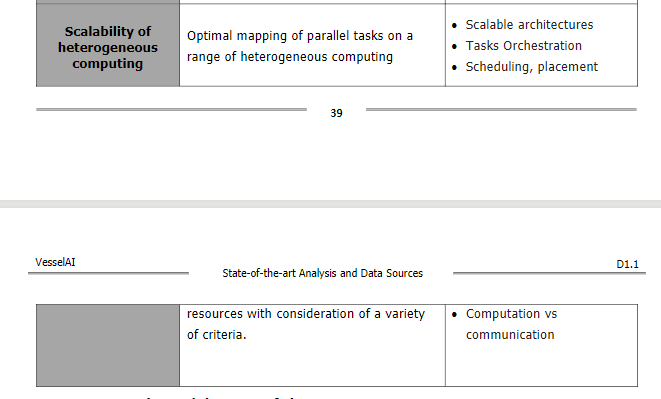
\includegraphics[scale=0.8]{hpciotchallengefromd11.png}

results summary

\section{chapter roles}
%3rd paragraph/section: chapter roles
The rest of the paper is organized as follows: 

Chapter 2 briefly describes state-of-the-art data applications' abstract components (the level will be like cleaning validating messaging storage and so on, very basics), widely established reference architectures (lambda and kappa at least). Also the systems evaluation dimensions (these are for example reproducibility, scalability, latency accuracy and fault tolerance) are defined. 

I also read some papers on the most established and non-sensor systems, like google millwheel and twitter storm, these could be briefly mentioned as examples on the dimension tradeoff choices and how they can impact the system. also the apache tools (kafka, hadoop) are mentioned a lot in literature so should they somehow be mentioned also

Also the general context for vesselai will be described. Specialities like data volume, spatial distribution of data sources and sensor-like+static data will be described. Also something on what AIS is and how the data is like. 

Chapter 3: bridge to this chapter: the previous context gives the following requirements: dissection on requirements comes here

the main point of this chapter is to go through systems that have similar requirements to vesselai, ie iot systems, maybe with special emphasis on smart cities because they also have spatial data and large volume. The question is which sensor systems are good for which dimension optimization and which set challenges on which dimension.

the second-last chapter:  the vesselai system
analysis, evaluation, experiences, recommendations, future improvement needs (these keywords from thesis instructions)
the architectural model of choice for vesselai, or 1-3 best options and their respective tradeoffs. Also discussion on what is reasonable to conclude: for example is the evidence solid enough to tell if edge computing is better than centralized, or
if stream and batch should be combined or not, and on which questions further experimentation and measurements are needed

conclusion
this part will generalize: what was learned from the vesselai conclusion that is applicable to extreme scale data systems in general?

\section{acm classification,  keyword ideas}

acm:
Information systems → Information systems applications →
Spatial-temporal systems → Data streaming (from \cite{uprctrajectorysystem})

end to end + sensor data (iot) + machine learning + maritime + inference + lifelong learning

Distributed Machine Learning, Internet of Things, Training, Serving (from \cite{mliot})

title wordplay:

Sensor data systems at extreme scale / for scale

% this portion currently: very very very drafty text on the topic, all this can be added -s from literature
\chapter{context}

\section{on machine learning}

anything used later that my level reader might not understand comes here

define federated learning and lifelong learning

\section{on big data systems in general}

to add here: a high-enough abstraction / "charting of the field" of big data systems in general

the high level components, d1.2 p 32 has one good starting point

definition of a user request in this context: the human is not considered, they use the ui. user is the application making requests to the system. these might be preprocessing-related or actual human user requests

\subsection{the Lambda and Kappa architectures}

% this is the content on lambda & kappa that is probably needed content-wise. only needs better writing.

the initial motivation behind lambda: to beat cap theorem's inherent need to tradeoff between consistency and availability \cite{lambdakappa}

nathan marz presenting a system that supposedly beats cap. how: treat data as immutable, emphasize importance of preparing for human error, and splitting a database into two systems, batch and speed layer. The batch layer does order of hours long preprocessing of queries, speed layer has  abstracted within itself a complex system for handling the data from the latest hours to make also that available for querying. Fault tolerance comes mainly from the fact that the speed layer is possible to empty to the batch queue and restart in case of failure or overload.

the most known criticism to lambda, a blog post by Jay Kreps \cite{questioninglambda}, acknowledged its strengths in seeing data as immutable and highlighting the possibility that data may be needed to reprocess due to changes in application code. The main points of criticism were the argument that lambda does not actually beat cap but still compromises some consistency, that deeming real-time stream processing as inherently faulty and approximate "does not make sense" and is only a fault in the current tools \cite{questioninglambda}. The post along with other sources deem the most important flaw in lambda to be the fact that maintaining and syncronizing separate code bases for batch and stream layer to be redundantly complex \cite{uber} \cite{facebook}. At the same time multiple system analyses name maintainability the most or one of the most important trait about a big data system \cite{facebook} \cite{storm@twitter}.

As an alternative approach to solve these problems, Kreps proposed a different architecture called the Kappa architecture. It is otherwise similar to lambda but only has either batch or speed layer, usually speed layer in a for of highly parallelized stream processor. This mitigates the duplication problem while keeping other strengths from lambda, but the ability of giving fast answers to queries is lost.

(\cite{D1.1} states that both lambda and kappa mitigate human errors ''by  updating  the  code  and  running  it  again  on  the historical  data '')

% problems with both lambda&kappa, structure needs reorder because this does not make sense before vesselai requirement specs

fundamental assumptions of both systems:  the need almost instant execution times is assumed \cite{lambdakappa}. This is not required in vesselai. also, not stated in the sources on lambda and kappa but still assumed: that we are able to tell before the user query what exactly is going to be queried. If in vesselai the model may change and with that the query as well, or more importantly the queries regard only a mini fraction of geographical space so preprocessing the full globe and needing a percent of the preprocessed has a potential of being a grande waste of computation in the maritime case (my judgement). for the latter point it is possible that neither lambda or kappa are good.

- all the apache systems: what they are what is each used for, a very short description


\section{the evaluation dimensions}

For this thesis, dimensions are defined as traits by which various systems can be evaluated. These are:

latency: the time it takes from user input until they get their desired output,

scalability: at which data volume per time unit the system faces bottlenecks,

accuracy: how true the predictions made by the system are and how much information the system is able to give its user about the predictions' accuracy.

throughput: how many user requests the system is able to handle (this trait may not be necessary)

a word for how easy something is to improve on...: multiple mature big data systems descriptions mentioned this as the most of one of the most important trait in the system \cite{uber} \cite{facebook}.

\section{note on hardware types}

something on how fast is fast, how powerful the hpc systems are compared to laptops

what are raspberry pi and arduino and how their power compares to a standard laptop

\section{vesselai case: detailed description}

% this paragraph: data description
The data is a combination of both descriptive static data, such as geographical information, and dynamic data. Dynamic data types are weather data and AIS, the Automatic Identification System data. The latter is the most important but also the most voluminous and erroneous. Maybe some examples here on what kind of errors ais has, like manually written distinations, location errors and illegal traffic disguising their action

% a paragraph for giving the vesselai high level architecture to show which part we are talking about (inference)
On the model library from d4.1; models etc will be located in the ai4eu catalog as docker containers \cite{D4.1}

The project is set out to solve ''in  particular  extreme-scale,  continuous  and  lifelong  learning  and  serving  of  AI  models'' \cite{D4.1}. This thesis is trying to find the best deployment scheme to enable meeting of perfomance requirements (latency, throughput, scalability) and facilitating lifelong learning.

\cite{D4.1} also has on page 15 an ok illustration on where the model library is in the system but a more high level one will probably be included here.

% this paragraph: requirements
% old text
The use cases for the vesselai project are named in four pilots, which are intelligent routing, ship energy systems design, autonomous vessel operating and weather routing. In terms of the dimensions of evaluation stated above this demands on scalability above all. Latency, correctness, and fault tolerance depend on the application: in highly congested areas an application for collision detection might set high demands on these. a routing application for multi-week journey: if a prediction is often not accurate a lot of fuel costs are added. The latency is still in every application in order of seconds even up to a minute for the user request and pre-processing can take time: weather data comes 4x a day for example. No instant-seeming action, ie milliseconds end to end time are required. Therefore they should not be aimed for as cutting down time will inevitably reduce quality in other, more critical dimensions.

%on time requirements
One fundamental difference of the maritime application domain compared to other applications are the time requirements: usually instant-seeming is required, ie order of milliseconds. In maritime, time requirements range from a few seconds up to 60 minutes (second to minute discussed in the napa meet for pilot 4, 30-60 in the uprc meet for pilots 1&3)

\chapter{vesselai-like systems}

\section{tradeoffs}

a tradeoff: federated vs centralized learning \cite{iotsurvey}

edge vs central inference: if on edge the model needs to be small \cite{iotsurvey}

is data cleaned before or after storage?

data semantics: should data be at least once, exactly once or at most once (duplicate cleanup speed vs quality). if cleanup happens after storage different applications can have different semantics

\chapter{the vesselai system}

i e the results i get
